\documentclass[10pt,oneside]{article}

\usepackage{amsfonts}
\usepackage{amsmath}
\usepackage{amssymb}
\usepackage{dsfont}
\usepackage{bm}

\usepackage{epsf}
\usepackage{epsfig}
\usepackage{graphicx}
\usepackage{wrapfig} \usepackage{subfig}

\usepackage{enumerate}
\usepackage{listings}

\usepackage{setspace}
\usepackage{geometry}
\usepackage{fancyhdr}
%\usepackage{soul} % cross out text

\usepackage[latin2]{inputenc}
% \usepackage{times} % ez kiszedi a t1enc raszteressgt, de valami ms betu"tpust
% hasznl
\usepackage{lmodern} % ez eltu"nteti a raszteressget s mg jk is a betu"k
% \usepackage[magyar]{babel}
\usepackage{t1enc}

% \usepackage[T1]{fontenc}

\usepackage[usenames]{color}
% \usepackage[colorlinks]{hyperref} \usepackage{showkeys}

% \onehalfspacing
\usepackage{indentfirst}
% \frenchspacing

\geometry{left=2.5cm,right=2.5cm,top=3.0cm,bottom=2.5cm}

\pagestyle{fancy}
\lhead{Bayesian parameter estimation}
\chead{ }
\rhead{\thepage}

\lfoot{ }
\cfoot{ }
\rfoot{P�ter K�m�r, \the\year}


\renewcommand{\headrulewidth}{0.4pt}
\renewcommand{\footrulewidth}{0.0pt}



% \numberwithin{equation}{section} \numberwithin{figure}{section}
% \numberwithin{table}{section}

\author{P\'{e}ter K\'{o}m\'{a}r}
\title{Methods of Bayesian Parameter Estimation}
\date{\today}





\begin{document}
\newcommand{\bel}{\begin{equation}}
\newcommand{\eel}{\end{equation}}
\newcommand{\be}{\begin{equation*}}
\newcommand{\ee}{\end{equation*}}

\newcommand{\bal}{\begin{eqnarray}}
\newcommand{\eal}{\end{eqnarray}}
\newcommand{\ba}{\begin{eqnarray*}}
\newcommand{\ea}{\end{eqnarray*}}

\newcommand{\ket}[1]{| #1 \rangle}
\newcommand{\Ket}[1]{\left| #1 \right\rangle}
\newcommand{\bra}[1]{\langle #1 |}
\newcommand{\Bra}[1]{\left\langle #1 \right|}

\newcommand{\no}{\noindent}

\newcommand{\ev}[1]{\langle #1 \rangle}
\newcommand{\Ev}[1]{\left\langle #1 \right\rangle}
\newcommand{\Tr}{\text{Tr}\,}
\newcommand{\+}{^\dagger}
\newcommand{\s}{^\ast}
\newcommand{\PP}{\mathcal{P}}
\newcommand{\eqE}{= \!\!\!\!\!^{{}^{E}}\,}

\renewcommand{\d}[1]{\!d #1 \;}

\newcommand{\bE}{{\mathbf E}}
\newcommand{\bB}{{\mathbf B}}
\newcommand{\bF}{{\mathbf F}}
\newcommand{\bJ}{{\mathbf J}}
\newcommand{\bv}{{\mathbf v}}
\newcommand{\eps}{\varepsilon}
\newcommand{\br}{\mathbf r}
\newcommand{\bk}{\mathbf k}
\newcommand{\hatx}{\hat{\mathbf{x}}}
\newcommand{\haty}{\hat{\mathbf{y}}}
\newcommand{\hatz}{\hat{\mathbf{z}}}

\renewcommand{\vec}[1]{{\bf #1}}
\newcommand{\mat}[1]{{\bf #1}}

\newcommand{\op}[1]{\mathbf{#1}}
\newcommand{\twovector}[2]{
	\left[
		\begin{array}{c}
		#1 \\
		#2
		\end{array}
	\right]
}
\newcommand{\threevector}[3]{
	\left[
		\begin{array}{c}
		#1 \\
		#2 \\
		#3
		\end{array}
	\right]
}
\newcommand{\fourvector}[4]{
	\left[
		\begin{array}{c}
		#1 \\
		#2 \\
		#3 \\
		#4
		\end{array}
	\right]
}
\newcommand{\fivevector}[5]{
	\left[
		\begin{array}{c}
		#1 \\
		#2 \\
		#3 \\
		#4 \\
		#5
		\end{array}
	\right]
}
\newcommand{\nvector}[2]{
	\left[
		\begin{array}{c}
		#1_1 \\
		#1_2 \\
		\vdots \\
		#1_#2
		\end{array}
	\right]
}
\newcommand{\ncovector}[2]{
	[#1_1\s, #1_2\s, \dots #1_#2\s]
}
\newcommand{\twobytwomatrix}[4]{
	\left[
		\begin{array}{cc}
		#1 & #2\\
		#3 & #4
		\end{array}
	\right]
}
\newcommand{\threebythreematrix}[9]{
	\left[
		\begin{array}{ccc}
		#1 & #2 & #3\\
		#4 & #5 & #6\\
		#7 & #8 & #9
		\end{array}
	\right]
}
\newcommand{\threebythreedeterminant}[9]{
	\left|
		\begin{array}{ccc}
		#1 & #2 & #3\\
		#4 & #5 & #6\\
		#7 & #8 & #9
		\end{array}
	\right|
}
\newcommand{\nbymmatrix}[3]{
	\left[ 
		\begin{array}{cccc}
		#1_{11}  & #1_{12} & \dots  & #1_{1 #2}\\
		#1_{21}  & #1_{22} &        &         \\
		\vdots   &         & \ddots & \vdots  \\
		#1_{#3 1}&         & \dots  & #1_{#3 #2}
		\end{array}
	\right]
}
\newcommand{\nbyndeterminant}[2]{
	\left|
		\begin{array}{cccc}
		#1_{11}  & #1_{12} & \dots  & #1_{1 #2}\\
		#1_{21}  & #1_{22} &        &         \\
		\vdots   &         & \ddots & \vdots  \\
		#1_{#2 1}&         & \dots  & #1_{#2 #2}
		\end{array}
	\right|
}


\newcommand{\argmax}[1]{\underset{#1}{\operatorname{arg}\operatorname{max}}\;}

%\thispagestyle{empty}
%\maketitle
 
%\newpage
%\tableofcontents


\lstset{
numbers=left, 
numberstyle=\small, 
numbersep=8pt, 
frame = single, 
language=Python, 
framexleftmargin=15pt
}


\section*{Bayesian inference}
\no When facing an inference problem that we wish to tackle with a Bayesian method, we start with the following steps.
\begin{enumerate}
	\item Collect the data $D = \{d_1, d_2, \ldots d_N\}$, where each $d_i$ can be a vector or even a matrix of observations, but each $d_i$ is independent from every other $d_j$ (given fixed model parameters).

	\item Come up with a generative model $P(d \,|\, \theta)$, where $\theta = (\theta_1, \theta_2, \ldots \theta_K)$ stands for the collection of all unknown model parameters.

	\item Use our best judgment to come up with a prior distribution for $\theta$, $P_0(\theta)$.

	\item Write down the posterior 
	\be
		P(\theta\,|\,D) = \frac{P_0(\theta) \prod_i P(d_i\,|\,\theta)}{Z} =  \frac{\tilde P(\theta\,|\,D)}{Z},
	\ee
	where $\tilde P(\theta\,|\,D)$ is the unnormalized posterior of $\theta$ and $Z$ is the necessary normalization factor (independent of $\theta$).

	\item Calculate or approximate relevant characteristics of the posterior. These often include
	\begin{itemize}
		\item median of each $\theta_k$, mean and mode of $\theta$,
		\item percentiles and standard deviation of each $\theta_k$, and covariance matrix of $\theta$,
		\item histogram of each $\theta_k$.
	\end{itemize}
\end{enumerate}

This 5th step is hard. Exact analytical solutions exist for a handful of widely-used models, most of which assume (multivariate) Gaussian distributions, and exact numerical solutions are feasible if model parameters are few, $K \lesssim 5 $. Most non-Gaussian, real-life inference problems, however, require approximations or sampling to carry out the 5th step.

\subsection*{Exact solutions}

\begin{itemize}
	\item {\bf Analytical.} In rare cases (typically Gaussian models), $Z$ can be expressed as an analytical formula of the data $D$, and the posterior $P(\theta\,|\, D)$ is a known distribution, the formulas for whose mean and variance can be looked up.

	\item {\bf Numerical.} If no analytical solution exists, one can numerically evaluate $w_\theta = \tilde P (\theta\,|\, D)$ on a \emph{regular} grid of $\theta$ values. Posterior distribution, expectation value and variance can be calculated as averages:
	\be
		P(\theta) \approx \frac{w_\theta}{\Delta\theta \sum_\theta w_\theta},\qquad \mathbb{E}(\theta) \approx \frac{\sum_\theta w_\theta\theta }{\sum_\theta w_\theta}, 
		\qquad \text{Var}(\theta) \approx \frac{\sum_\theta w_\theta \theta^2 }{\sum_\theta w_\theta} - \left[\mathbb{E}(\theta)\right]^2,
	\ee
	where $\Delta \theta$ is the volume of a grid cell on the regular $\theta$ grid.
	Median, mode and covariance can also be directly evaluated from the posterior, $P(\theta)$.
	This is feasible only if the dimension of $\theta$, i.e. K,  is small. Making the grid finer makes this approximation more accurate.
\end{itemize}

\subsection*{MCMC sampling}
As the dimension of $\theta$ increases, evaluating $\tilde P$ on a regular grid becomes unrealistic. This is called the curse of dimensionality. Monte-Carlo Markov Chain (MCMC) sampling provides an alternative strategy: Instead of scanning all values of $\theta$ and weighting them with their (unnormalized) posterior value $w_\theta$, MCMC methods obtain samples from the posterior. 

The most notable MCMC sampling methods are {\bf Metropolis-Hastings} sampling, {\bf Hamiltonian} sampling and {\bf Gibbs} sampling.
Common to all sampling methods, they produce a series of $\theta^{(t)}$ samples for $t = 0, 1, \ldots T$, drawn approximately from the posterior $P(\theta\,|\,D)$. Methods differ in how they draw $\theta ^{(t+1)}$ using $\theta^{(t)}$ and the data $D$. All MCMC methods have a warm-up time $t_0$, during which samples are similar to the starting value $\theta^{(0)}$, and a thinning period $\tau$, which sets the minimal necessary distance between samples so they are not correlated significantly. From the resulting samples, expectation value and variance can be approximated as
\be
	\mathbb{E}(\theta) \approx \frac{1}{L}\sum_{l=1}^L \theta^{(t_0 + l\tau)},
	\qquad
	\text{Var}(\theta) \approx \frac{1}{L}\sum_{l=1}^L \left[\theta^{(t_0 + l\tau)}\right]^2 - \left[\mathbb{E}(\theta)\right]^2,
\ee
where $L = (T - t_0) / \tau$ is the total number of (approximately) uncorrelated samples. Median, mode and covariance can also be directly approximated by their empirical values from the samples $\{\theta^{(t_0 + l\tau)}\,:\;l=1,2\ldots L\}$.

To find acceptable values for warm-up time $t_0$, we can plot traces of $\theta^{(t)}$ as a function of $t$. We should choose $t_0$ such that all initial transient motion is gone for $t > t_0$. The thinning period can be choosen by plotting thinned traces $\theta^{(t_0 + l\tau)}$ as a function of $l$ for different $\tau$ values, and choosing the smallest $\tau$ for which the line-plot of the trace looks like a ``hairy caterpillar''.

{\bf Disclaimer:} MCMC sampling methods are prone to the problem of isolated local maxima in the posterior: If two or more regions of the posterior are equally likely but separated by deep valleys, no sampler will be able to make jumps between them. To mitigate this, running multiple chains, started from different $\theta^{(0)}$ values can be run. We can monitor the log-posterior $\log \tilde P(\theta^{(t)}\,|\,D)$ for each chain, which, if it is significantly lower than the other chains, indicate that the chain in question is stuck in a sub-optimal local maximum. Then we can discard it, and combine the samples only from chains that have similarly high log-posterior.

\subsection*{MAP + Laplace approximation}
MCMC sampling methods require drawing a new sample $\theta^{(t+1)}$ in every iteration, for which the algorithm needs to have efficient access to all data $D$. This becomes a logistic difficulty as the size of the data $N$ increases, resulting in slowdown. Sampling methods are practical only for inference problems, where the data (not the raw data, but the features relevant for the inference problem) fit comfortably in memory. When both exact methods and sampling methods prove to be infeasible, maximum a posteriori (MAP) estimation combined with Laplace approximation may provide acceptable solutions. 

Strictly speaking MAP finds only the mode of the posterior distribution,
\be
	\theta_\text{MAP} = \text{mode}(\theta) = \arg \max_\theta \left[\tilde P(\theta\,|\,D)\right] = \arg \max_\theta \left[\log \tilde P(\theta\,|\,D)\right].
\ee
This can be calculated by one of the following methods.
\begin{itemize}
	\item {\bf Analytically}, if the unique solution to the algebraic equations, 
	\be
		0 = \partial_{\theta_k} \log \tilde P(\theta\,|\,D)\qquad k=1,2\ldots K,
	\ee
	can be found in closed form.

	\item {\bf Gradient descent} starts from $\theta^{(0)}$, and continually moves $\theta$ towards the direction in which $-\log \tilde P(\theta\,|\, D)$ is decreasing most steeply. This is implemented by python's \texttt{scipy.optimize.minimize()} function.

	\item {\bf Expectation-Maximization methods} separate the parameters in $\theta$ into two groups (usually: latent variables and model parameters), in such a way that allows one-step optimization of one group while the other is fixed. Alternating which group to fix and which to optimize, eventually, results in converging to a local maximum of the log posterior.
\end{itemize}

Laplace approximation can always be carried out, after the MAP estimation is found. It approximates the posterior with a Gaussian distribution centered at the MAP estimate. The covariance of this Gaussian is
\be
	\text{Cov}_\text{Laplace}(\theta) = \Big[-\nabla_\theta \nabla_\theta \log \tilde P(\theta\,|\,D)\Big]^{-1},
\ee
i.e. the inverse of the negative second-order derivative (aka Hessian matrix) of the log posterior. For 1-dimensional $\theta$, it gives a single number, the ``Laplace variance'' of $\theta$.


\newpage
\section*{Example}
The hand of an assembly-line robot needed to be replaced 31 days, 82 days, 122 days and 186 days after its initial purchase. Question: What is the estimated lifetime of the robot's hand?

\subsection*{Data and Model}
The data consists of $N = 4$ waiting times between consecutive installations:
\be
	D = \{t_1, t_2, t_3, t_4\} = \{31 - 0, 82 - 31, 122 - 82, 186 - 122\} = \{31, 51, 40, 64\}.
\ee

Assuming that the workload was constant, we model $t_i$ with an exponential distribution with lifetime of $\tau$ days.
\be
	P(t\,|\,\tau) = \frac{1}{\tau} \exp\left(-\frac{t}{\tau}\right).
\ee

We use an uninformative prior for the lifetime:
\be
	P_0(\tau) = \frac{\text{const.}}{\tau},
\ee
where const. stands for an appropriate constant that normalizes the prior in a plausible region.

The posterior can be written as
\be
	P(\tau\,|\, D) = \frac{P_0(\tau)\prod_i P(t_i\,|\,\tau)}{Z} = \frac{1}{Z}\frac{1}{\tau} \prod_i \left[\frac{1}{\tau} \exp\left(-\frac{t_i}{\tau}\right)\right] = \frac{1}{Z}\frac{1}{\tau^{N+1}} \exp\left(-\frac{1}{\tau}\sum_i t_i\right).
\ee

\subsection*{MAP + Laplace approximation}
The unnormalized log-posterior is
\be
	\log \tilde P = \log\left[P_0(\tau)\prod_i P(t_i\,|\,\tau)\right] = - (N+1)\log \tau - \frac{\sum_i t_i}{\tau} + \text{const.}
\ee
Requiring that the first derivative is zero yields an algebraic equation for $\tau$, which we can solve for the MAP estimate, $\tau_\text{MAP}$.
\be
	0 = \partial_\tau \log\tilde P = -\frac{N+1}{\tau} + \frac{\sum_i t_i}{\tau^2}\qquad \Rightarrow \qquad \tau_\text{MAP} = \text{mode}(\tau) = \frac{\sum_i t_i}{N+1} = 37.20
\ee
The second-order derivative allows us to calculate the ``Laplace standard deviation'' $\text{std}_\text{Laplace}(\tau)$.
\ba
	(\partial_\tau)^2 \log\tilde P &=& \frac{N+1}{\tau^2} - \frac{2\sum_i t_i}{\tau^3} = - \frac{\sum_i t_i}{(\tau_\text{MAP})^3} \\
	\text{Var}_\text{Laplace} &=& \Big[- (\partial_\tau)^2 \log\tilde P\Big]^{-1} = \frac{(\tau_\text{MAP})^3}{\sum_i t_i} \qquad \Rightarrow \qquad \text{std}_\text{Laplace}(\tau) = \sqrt{\frac{(\tau_\text{MAP})^3}{\sum_i t_i}} = \frac{\sum_i t_i}{\sqrt{(N+1)^3}} = 16.64
\ea


\newpage
\subsection*{MCMC sampling}
Let's use STAN (http://mc-stan.org/) to run Hamiltonian sampling. The python API (pystan) is great. Let's run 4 chains with the NUTS algorithm, each with a total of 2000 iterations, the first 1000 of which we drop, but keep every one of the remaining samples. Here is the full code.

\lstinputlisting{Lifetime-stan.py}
\vspace{5mm}

Line 21 compiles the STAN model, defined by Lines 6-20, then it runs the sampling (Lines 26-32) and displays the results: the estimated mean and standard deviation of $\tau$ (Lines 36-37),
\begin{lstlisting}
mean(tau): 62.845930336113604
std(tau):  41.65566288308886
\end{lstlisting}

and an estimate of the posterior and traces of $\tau$ in the figure tau.pdf (Line 38).
% \begin{figure}[h]
% \centering
% 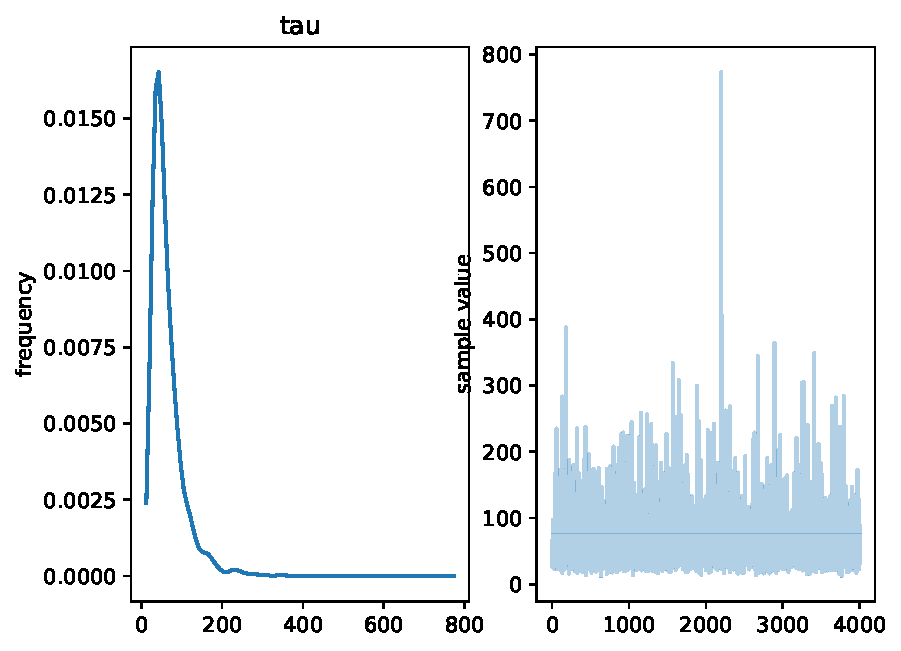
\includegraphics[width=0.5\textwidth]{./tau.pdf} 
% \caption{tau.pdf produced by the pystan code.}
% \end{figure}


\newpage
\subsection*{Exact solution}
The normalization constant $Z$ can be calculated by integrating the unnormalized posterior over the entire domain of $\tau$ (here we apply the limits $\tau_\text{min} \rightarrow 0$ and $\tau_\text{max} \rightarrow \infty$ to obtain closed forms):
\be
	Z = \intop_0^\infty\d{\tau} \frac{1}{\tau^{N+1}} \exp\left(-\frac{1}{\tau}\sum_i t_i\right) = \frac{1}{\left[\sum_i t_i\right]^{N}} \intop_0^\infty \d{z} z^{N-1} \exp(-z) = \frac{\Gamma(N)}{\left[\sum_i t_i\right]^{N}},
\ee
where we used a new variable $z = \frac{1}{\tau}\sum_i t_i$, and expressed $\tau = \frac{1}{z}\sum_i t_i$ and $d\tau = -\frac{dz}{z^2}\sum_i t_i$. The analytical form of the normalized posterior is
\be
	P(\tau\,|\,D) = \frac{\left[\sum_i t_i\right]^{N}}{\Gamma(N)} \tau^{-N-1} \exp\left(-\frac{\sum_i t_i}{\tau}\right) = \frac{\beta^{\alpha}}{\Gamma(\alpha)} \tau^{-\alpha-1} \exp\left(-\frac{\beta}{\tau}\right) = \text{IG}(\tau\,|\,\alpha, \beta),
\ee
which is the inverse-gamma distribution for $\alpha = N$ and $\beta = \sum_i t_i$, the mean, mode and standard deviation are
\ba
	\mathbb{E}(\tau) &=& \frac{\beta}{\alpha - 1} = \frac{\sum_i t_i}{N-1} = 62.00\\
	\text{mode}(\tau) &=& \frac{\beta}{\alpha + 1} = \frac{\sum_i t_i}{N+1} = 37.20\\
	\text{std}(\tau) &=& \frac{\beta}{(\alpha -1)\sqrt{\alpha -2}} = \frac{\sum_i t_i}{(N-1)\sqrt{N-2}} = 43.84
\ea

\subsection*{Comparison}
We can plot the posterior densities, produced by the three methods. While the histogram of the Monte Carlo Markov Chain samples (Line 35 in code) reproduce the exact posterior quite well. The MAP + Laplace approximation is accurate only in finding the mode and estimating the order of magnitude of std, but it fails to capture the skewness of the posterior, and underestimates $\tau$.
\begin{figure}[h]
\centering
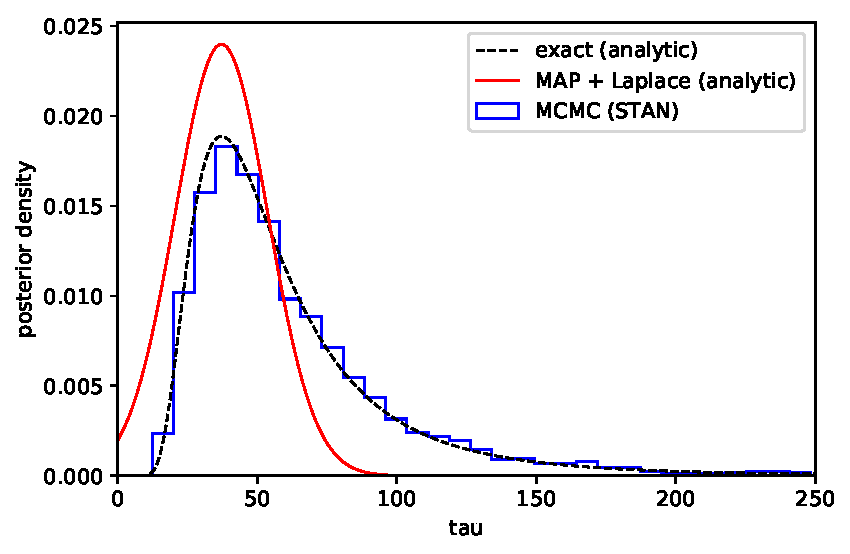
\includegraphics[width=0.7\textwidth]{./tau_posterior.pdf} 
\caption{Posterior of $\tau$ as estimated by MAP + Laplace approximation and MCMC sampling, as well as the exact curve.}
\end{figure}


\newpage

\section*{Problems}
All of the following problems can be solved with MCMC sampling. Apart from one, they are also solvable with MAP+Laplace approximation, either analytically or numerically. Several of them also have exact analytical solutions. In each problem, we are interested in a ``best guess'' (e.g. mean or mode) and some ``error bars'' (e.g. std) for the parameters in question.

\subsubsection*{Problem 1 - Linear regression}
Given $(x,y)$ data ($x = [1,2,3,4,5,6,7], y = [3.23, 5.38, 6.54, 7.99, 9.86, 11.35, 11.98]$), assume a linear model $y = ax + c + \varepsilon$, where $\varepsilon$ is a Gaussian variable with zero mean and variance $\sigma^2$. Estimate the parameters $(a, c, \sigma^2)$.

\subsubsection*{Problem 2 - Negative binomial}
An experiment with binary outcome is performed until it fails $r = 5$ times; the recorded number of successes is $k = 21$ (see negative binomial distribution). Estimate the success probability $p$.

\subsubsection*{Problem 3 - Normal}
A person took seven different IQ tests and got the following scores, $x = [112, 111, 115, 131, 124, 114, 96]$. Assume normal distribution of the test results $x \sim \mathcal{N}(\mu, \sigma^2)$, and estimate the parameters $(\mu, \sigma^2)$. What is the probability that $\mu$, is below 100?

\subsubsection*{Problem 4 - Fixed effect model}
In a greenhouse, tomato plants are separated into three (unequal) groups, each of which is treated with a different fertilizer. Yield of each plant, $y$ (in grams) is measured to be
\ba
	\text{group A:}&& y_A = [2604, 2665, 2251, 2510] \\
	\text{group B:}&& y_B = [1559, 1729, 1866, 1414, 1159, 1692] \\
	\text{group C:}&& y_C = [1528, 1444, 1041] 
\ea
Let's model yield as $y_{g,i} = \mu_g + \varepsilon_{g,i}$, where $g\in \{A,B,C\}$ is the group index, $i = 1,2,\ldots$ is the plant index, $\mu_g$ are fixed and unknown, and $\varepsilon_{g,i}$ are iid. Gaussian variables with zero mean and $\sigma^2$ variance. Estimate the parameters $(\mu_A, \mu_B, \mu_C, \sigma^2)$.

\subsubsection*{Problem 5 - Random effect model}
Model the data in pProblem 4 as $y_{g,i} = \mu + \delta_g + \varepsilon_{g,i}$, where $\mu$ is fixed and unknown, $\delta_g$ are iid. Gaussian variables with zero mean and variance $\sigma_\delta^2$, and $\varepsilon_{g,i} \sim \mathcal{N}(0, \sigma^2)$ iid. as before. Estimate the parameters $(\mu, \sigma_\delta^2, \sigma^2)$. What percentage of the observed variance is explained by the difference in fertilizers, i.e. what is $\sigma_\delta^2 / (\sigma_\delta^2 + \sigma^2)$?

\subsubsection*{Problem 6 - $\exp(-x^4)$}
In a park, the heights of 10 pine trees are measured $x = [435, 491, 620, 356, 443, 398, 383, 475, 554, 639]$ in centimeters. Assume the following distribution for the heights,
\be
	P(x\,|\, c, s) = \frac{1}{Z}\frac{1}{s} \exp\left(-\frac{(x - c)^4}{s^4}\right),\qquad \text{where }Z = \frac{\Gamma(\frac{1}{4})}{2} = 1.8128,
\ee
and estimate the parameters $(c,s)$. [Extra: Fit a normal distribution too, and calculate which model has higher likelihood.]

\subsubsection*{Problem 7 - Uniform}
A pseudo-random number generator produces the following sequence $x = [8.155, 6.272, 3.583, 7.096, 6.469]$. Assume that it draws samples uniformly from an interval $l\leq x \leq h$, and estimate the parameters $(l, h)$.

\subsubsection*{Problem 8 - Mixed error profile}
Twelve screws produced by a machine are sent to quality control, and measured how much their length deviates from the specification. The measured deviations are $x = [$ -1.32, -8.17, -0.21, -0.73, +5.78, +1.75, -0.29, -0.34, -0.52, +1.29, -0.60, +0.28$]$ in percentages. We suspect that some unknown fraction ($f$) of the screws are affected by a much larger errors than the rest, and we model this with the following mixture distribution,
\be
	P(x\,|\,f, \sigma, s) = (1-f)\times\text{Normal}(x\,|\,0,\sigma) + f\times\text{Cauchy}(x\,|\,0,s) 
	= (1-f)\frac{1}{\sqrt{2\pi\sigma^2}}\exp\left(-\frac{x^2}{2\sigma^2}\right) + f \frac{1}{s\pi}\frac{1}{1 + (x/s)^2}.
\ee
Estimate the parameters $(f, \sigma, s)$. [Extra: For each measured deviation, estimate the probability that it is a result of the Cauchy-distributed error.] 

\subsubsection*{Problem 9 - Multinomial}
In an egg-processing unit, the quality control mechanism takes 20 eggs from the conveyor belt, and grades their quality, i.e. giving them labels A, B, C, D or F. The observed counts are $(n_A, n_B, n_C, n_D, n_F) = (7, 8, 3, 1, 1)$. Assuming multinomial distribution, estimate the fractions of each quality grades in this batch, i.e. the parameters $(p_A, p_B, p_C, p_D, p_F)$.

\subsubsection*{Problem 10 - Threshold effect}
In a school district, 3955 seniors took a standardized math test. The histogram of the scores are published, as shown below. 
A striking feature of this data is that no students received scores below 20. This is likely an indication that the minimal passing score was 20, and grading was done in a way that ensured that no student failed. This hypothesis is also supported by the visible abundance just above the score 20. 
\begin{figure}[h]
\centering
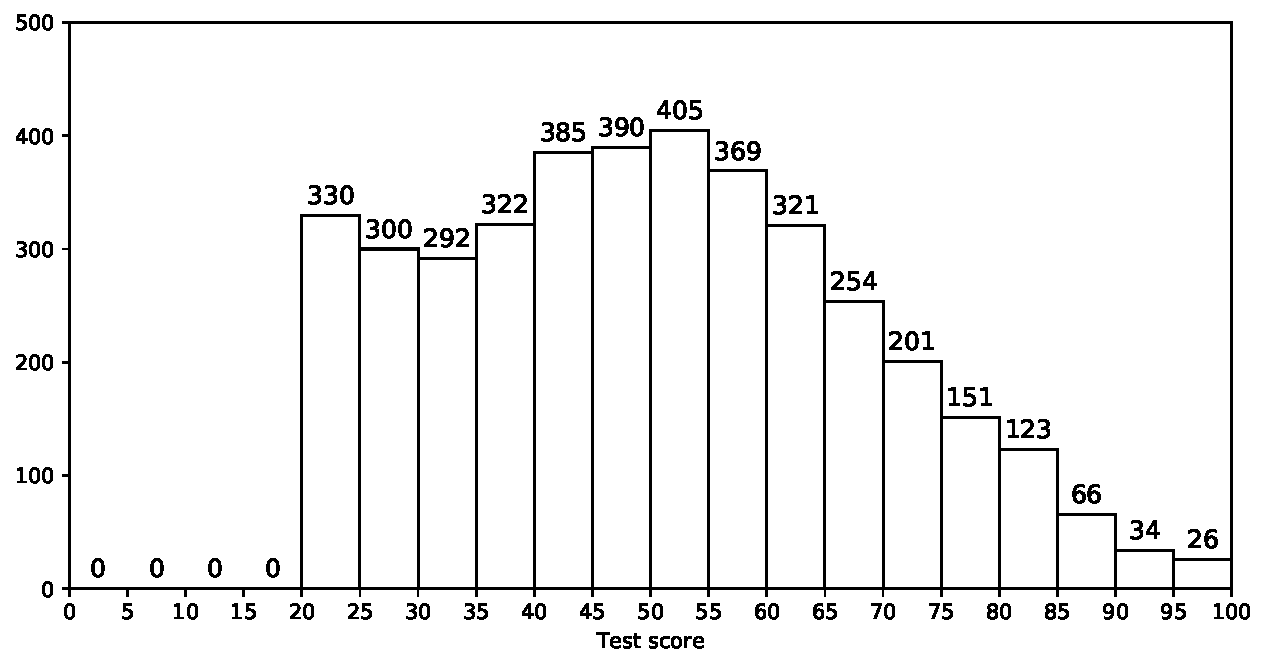
\includegraphics[width=0.6\textwidth]{test-scores.pdf}
\end{figure}


Let's estimate the distribution of the ``unadjusted'' scores by assuming the following process.
\begin{itemize}
	\item True scores are distributed according to a normal distribution with mean $\mu$ and standard deviation $\sigma$, truncated to the $[0,100]$ interval.

	\item If the true score is below 20, it gets adjusted. Let's model this by a replacement of the true score a score drawn from an exponential distribution with scale parameter $b$, truncated to the [20, 100] interval.
\end{itemize}
Estimate the parameters $(\mu, \sigma, b)$, and the proportion of the students that would have failed if their scores had not been adjusted.


















\end{document}